\documentclass[../main.tex]{subfiles}
\begin{document}
\tikzstyle{container} = [draw, rectangle, inner sep=0.3cm, dashed, minimum height=3.5cm]
In the last 50 years car have transitioned from being composed only by mechanical parts to being completely stacked with electronics. The complexity of vehicles arises every year and the industry continuously raise the bar on the state of the art. The transitions to electro-mobility, the ADAS systems have done all but slowing down the development. The more a topic is market relevant, the higher the competition between companies, the faster the development in that field is going to be. The automakers are always ready to exploit or create new needs in order to adapt and attract customers. Automotive pulse of innovation and the "German Silicon Valley" is the place a engineer want to be to fell part of this complex, but for sure perfectly oiled, machine.   
\begin{figure}
\centering
\begin{minipage}{.5\textwidth}
  \centering
  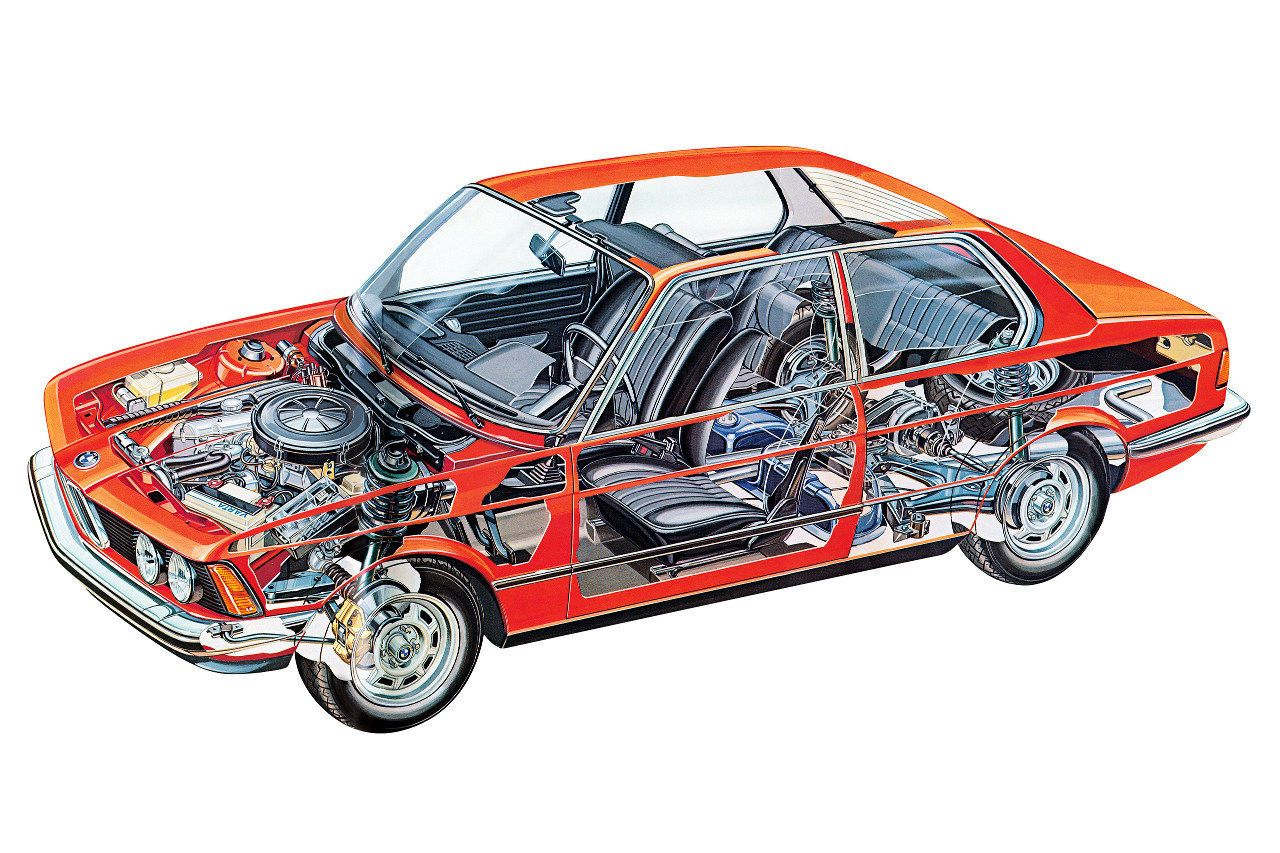
\includegraphics[width=\linewidth]{images_folder/4a56e1d50b56da42a10e29d451cf2b93.jpg}
  \caption{BMW 320 Coupe - 1975}
  \label{fig:test1}
\end{minipage}%
\begin{minipage}{.5\textwidth}
  \centering
  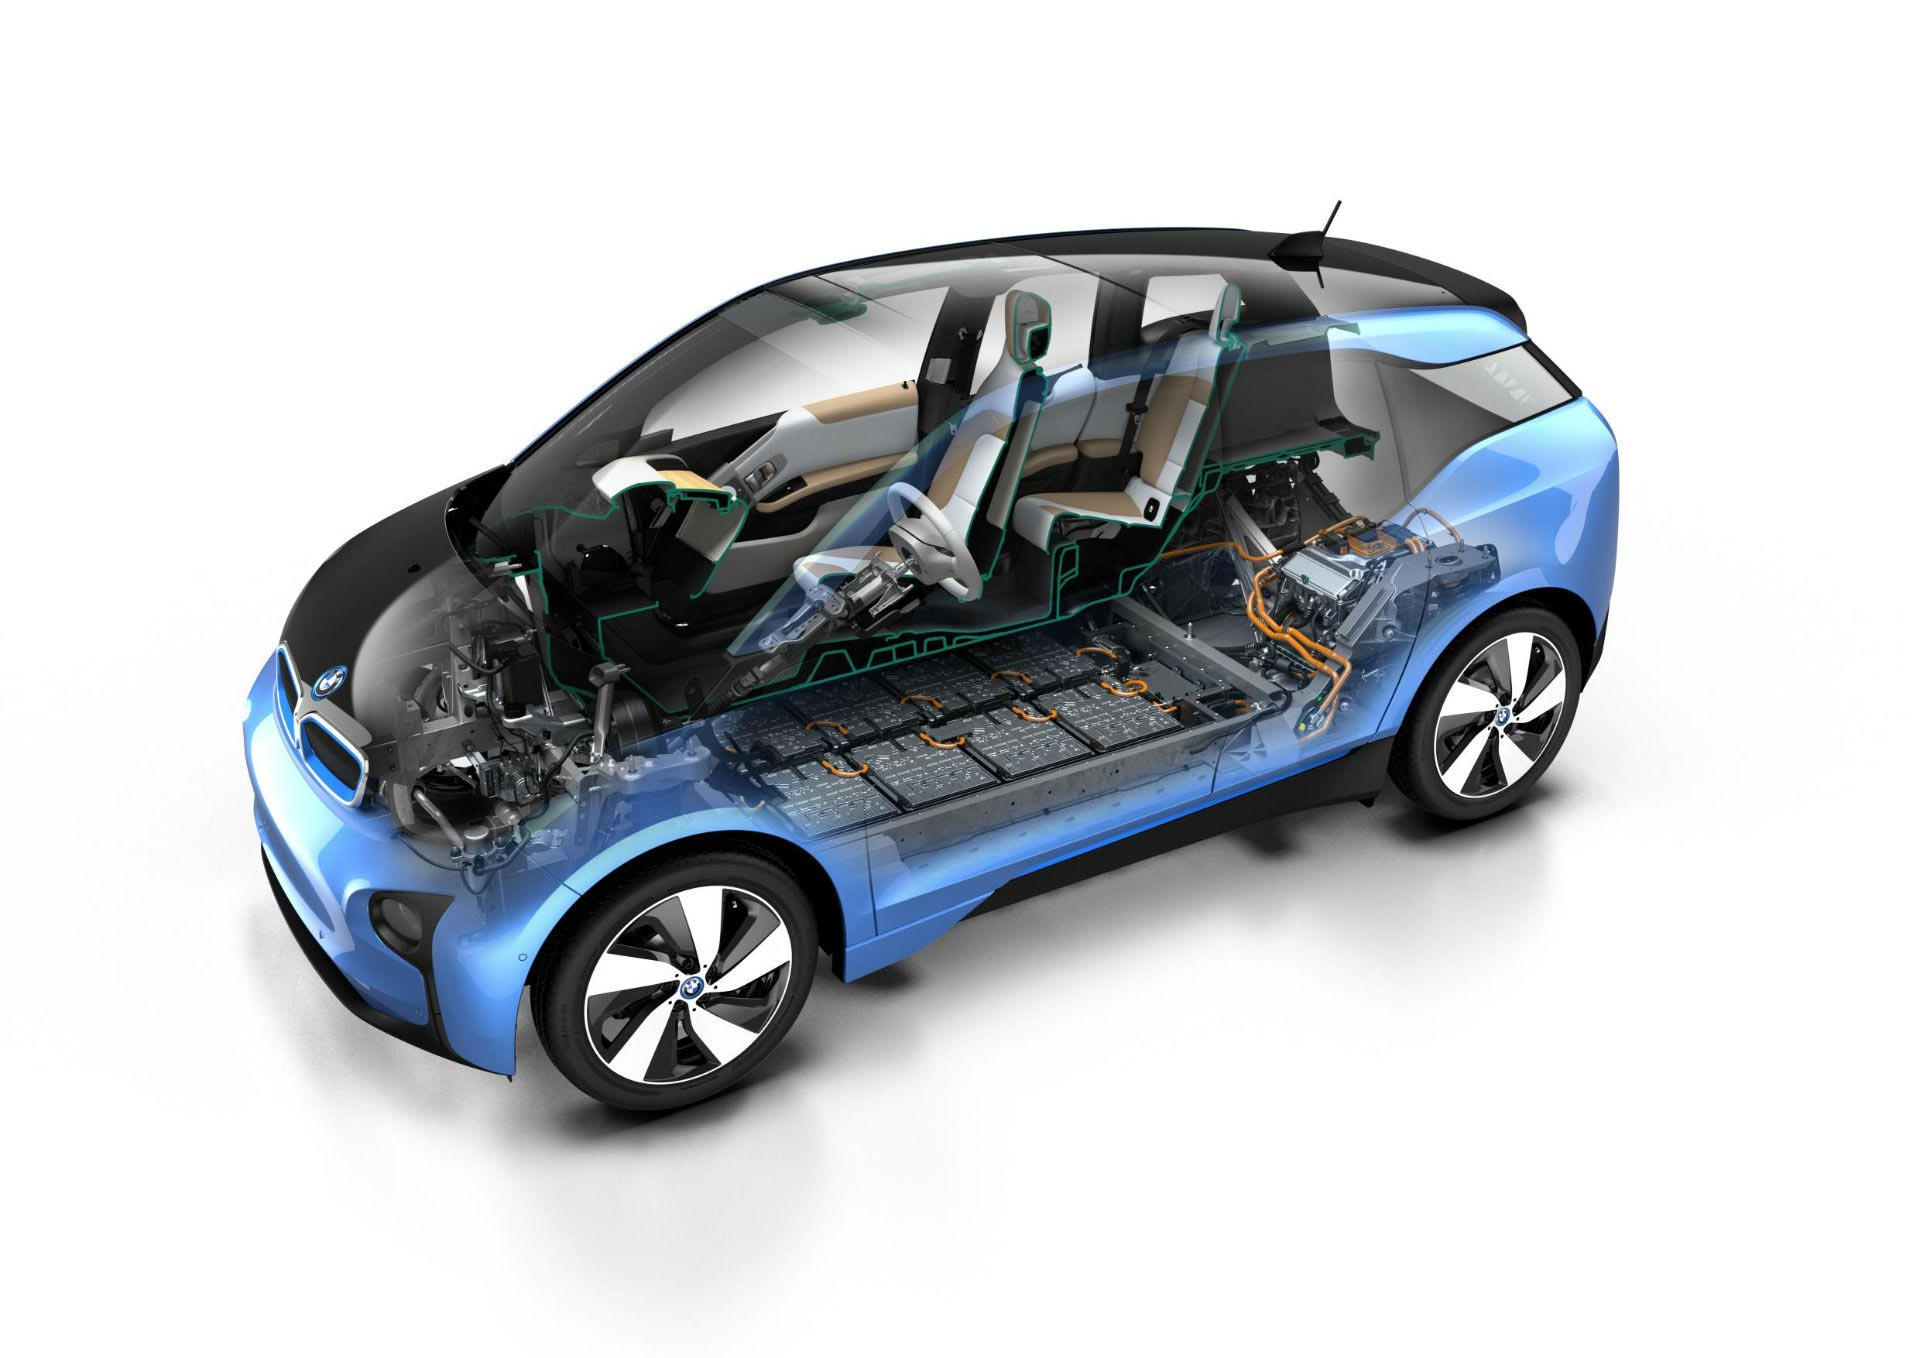
\includegraphics[width=\linewidth]{images_folder/BMW_i3.jpg}
  \caption{BMW I3 - 2015}
  \label{fig:test2}
\end{minipage}
\end{figure}

\section{Block Schema of a car}
The complexity of system car can be easily simplified by block schemes. Block schemes are going to be a recursive topic during the thesis, thanks to the outside view that they allow to have on complex topics. 
    \begin{figure}[ht]
        \begin{center}
  \begin{tikzpicture}[auto, node distance=3cm,>=latex', scale=0.7,transform shape]
            \node [input1, name=input] {};
            \node [sum1, right=of input] (sum) {};
            \node [block1, right=of sum] (controller) {$Vehicle \;System$};
            \node [output, right=of controller] (output) {};
            \draw [draw,->] (input) -- node {$User\; inputs$} (sum);
            \draw [->] (sum) -- node {} (controller);
            \draw [->] (controller) -- node [name=y] {$(speed,\; position..)$}(output);
            \draw [->] (y) -- ++ (0,-3) -| node [pos=0.99] {$-$} (sum);
            \end{tikzpicture}
        \end{center}
    \caption{Block Scheme of a car}
    \end{figure}
 
The input to the \textit{vehicle system} can be an array of driver commands, such as the steering, throttle position and all the settings that control the car. The output of the system is not only the movement of the car, but also more driver specific feeling such as the drive comfort or just the temperature in the vehicle. The \textit{vehicle system} can be further inspected, exposing two other block that are basic in the vehicle, the one responsible for the electronics and the one responsible for the mechanics. 
     \begin{figure}[ht]
        \begin{center}
  \begin{tikzpicture}[auto, node distance=3cm,>=latex', scale=0.7,transform shape]
            \node [input1, name=input] {};
            \node [sum1, right=of input] (sum) {};
            \node [sum, right=of sum] (sum_A) {};
            \node [block, right=of sum_A] (controller) {$Electronics$};
            \node [block, right=of controller] (mechanics) {$Mechanics$};
            \node [output1, right=of mechanics] (output) {};
            \draw [draw,->] (input) -- node {$User\; inputs$} (sum);
            \draw [->] (sum) -- node {} (sum_A);
            \draw [->] (sum_A) -- node {} (controller);
            \draw [->] (controller) -- node {} (mechanics);
            \draw [->] (mechanics) -- node [name=y] {$(speed,\; position..)$}(output);
            \draw [->] (mechanics) -- ++ (0,-2) -| node [pos=0.99] {$-$} (sum_A);
            \draw [->] (y) -- ++ (0,-4) -| node [pos=0.99] {$-$} (sum);
            % \node [container,fit=(controller) (mechanics) (sum_A)] (container) {};
            \end{tikzpicture}
        \end{center}
        \caption{'Sub block division'}
    \end{figure}       
These two blocks are strictly interconnected. The electronics drive the mechanics which output is given back as a feedback to correct the response. Continuing with the analogies, the system vehicle can be considered as a complex version of an embedded system where electronics drive mechanics following a logic described in lines of code.
Every mechanical component in cars has probably some electronic hardware related to it which is controlled by one of the many ECUs (Electronic control Units) in the vehicle. The increasing presence of embedded devices in the vehicle required a rapid increase in the software in order to control it. The yearly increase in lines of code for cars reported in \ref{fig:yearlyincreas} is a statement supporting of the importance of software. 
\begin{figure}[H]
    \centering
    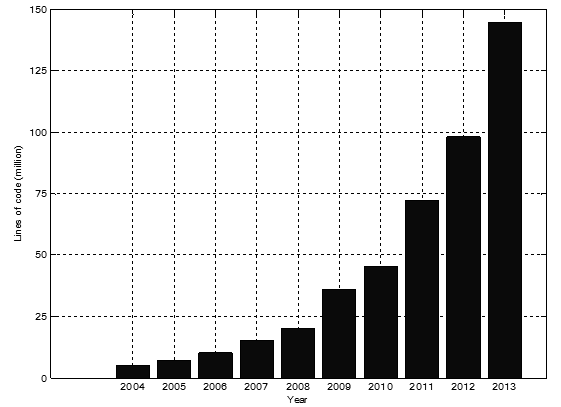
\includegraphics[width=0.6\linewidth]{images_folder/Yearly-increase-in-automotive-software-complexity-shown-by-million-lines-of-code-of-1-ConvertImage.png}
    \caption{Yearly increase in automotive software complexity}
    \label{fig:yearlyincreas}
\end{figure}
The fact that line of code are increasing mean a increasing complexity in the development process, which translate to requirement of a higher scalability and portability during the whole development process. The main in the thesis is going to focus on how this software is developed, generated and adapted to different ECUs. 
\section{Software and ECUs}
The development of Software for ECUs is an extremely complex task, a single ECU can control up to a 1000 functions, and the number can be also higher for the control of complex systems, such as the motor. The other big problem is that the function need to be developed in order to work together 
\cleardoublepage
\end{document}